\documentclass{article}

\usepackage{amsmath}
\usepackage{graphicx}
\usepackage{hyperref}
\usepackage{appendix}
%\newcommand{\pd}[2][]{\frac{\partial#1}{\partial#2}}

\title{\textbf{Temperature of Output Layer rather than Distillation Technique Determines the Robustness of Convolutional Neural Networks against Adversarial Perturbations}}
\author{Haobei Song \\
        University of Waterloo}
\date{March 26 2017}
\begin{document}

\maketitle
\pagenumbering{gobble}
\newpage
\pagenumbering{arabic}

\begin{abstract}
	Convolutional neural network (CNN) as a well developed deep learning architecture has been widely used in computer vision such as automatic inspection, autonomous driving, image processing. 
	Though state-of-art accuracy by elaborately designed CNN was achieved in many computer vision tasks, 
	recent studies have shown the potential vulnerability to adversarial perturbations among not only CNN but other deep neural networks.
	This discovery is of substantial significance as the widely usage of Convolutional neural network targets tasks of extensive security concern
	such as the CNN used in autonomous driving where the car might be crushed by slight modification of the environment. 
	In this study, the defensive effect of distillation training for CNN is evaluated together with traditional trained CNN for MNIST task on a data set of 60,000 examples.
	The result shows it is the temperature (T) of the softmax function of the output layer that plays an important role to reduce the adverserial gradient (by a factor of $10^{10}$ at $T=20$) and the success rate of adversarial attack (by a factor of 10 when $T=20$),
 rather than the distillation traininng technique claimed effective by other researchers.
\end{abstract}
\section{Introduction}
Considering when humans learn to recognize the digits written on a piece of paper, the input is the "viewing" of that image or the pixels on the paper with someone by their side teaching them the right number that image represents.
When people teach a computer how to do this by letting it learn the parameters characterizing such a task from a mass of data (hand written digits with labels) without explicitly crafting the algorithm, 
a general neural network is always built with some initial parameters to be modified to fit the given data set and generalize well when applied to new data. Learning the hand written digits is a classical deep learning task widely refered to as MNIST, which is often done by convolutional neural networks (CNN).

Ever since the introduction of convolutional neural networks for image processing tasks, the recognition accuracy has increased dramatically and achieved state-of-art accuracy in the past few years. Though computers now could outperform humans on this specific task,
recent study has shown the lack of robustness of CNN againt adversarial perturbations which raises plenty of problems about its pragmatic application. 

Compared with training computers to solve MNIST problem, humans during training process could learn more information than the hard labels given, such as the similarities between different digits, 
which is some information left out by traditional training with hard label. 
Theoretically, a deep enough neural network could learn such extra information when trained on a large enough scale of data. Such a neural network does not exist so far due to the limited data people can obtain and computation constraint required to perform the training on such neural network, as there is considerable complexity even within the simplest learning task such as MNIST. Humans often make use of knowledge from a variety of areas such as math, culture or even their personal experience to deal with MNIST tasks. For example, people can easily recognize rotated hand-written digits right after the training of upright digits from geometry or arabs could find some correlation from their language etc.
Thus, specifiing some hyperparameters of the training model is considerably neccesary for building a DNN to sole a realistic problem.

Though soft label method during training process has been suggested but crafting such soft label is also questionable as there is no general rule to create labels which perimetrize the relationship of hand-written digits falling into different categories as percieved by humans.
It also requres a considerable amount of effort to do these tedious task without a systemetic rule, which disabeys the principle of machine learning that simply tries to avoid these tedious work.

That is where distillation comes to the stage as to provide distilled labels from previously built CNN. The distilled labels can be considered as a kind of soft labels produced by computer, which labels each sample with a soft label using a traditional CNN. 
Papernot, McDaniel and Wu etc. have claimed its effectiveness against adversarial perturbation from empirical study in \cite{Papernot}.
In their work, they also applied a softmax output layer parametrized by a parameter called temperature, which turned out to be the most important factor reducing the success rate of adversarial attack in our study and the effectiveness of distillation solely becomes suspectable.

From a set of distilled labels, a deep learning neural network can gain more information such as the relationship between different handwritten digits explicitly. However, the information extracted by the previously built CNN is indeed part of information of the dataset training that CNN.
As a result, the distillation training method places a considerably rigorous requirement on the CNN that produces those distilled labels.
Theoretically, CNN built upon distilled labels can never outperform the previously built CNN either in prediction accuracy or robustness against adversarial perturbations based on the assumption that these CNNs make best use of every sample in the dataset. 
Though, it is of appreciable pragmatic significance as in reality, the dataset is always limited and the computational ability is just a trace of that of a human.
That is why distillation is initially used to train a deep learning neural network on a comparablly computational resource limited devices such as phones, which can then use the preprocessed or distilled labels produced from a DNN on a much powerful computer.

In this paper, we investigated the effectiveness of distillation applied to the classical MNIST classification problem as a defense to adversarial perturbations. We adopted three different algorithms to craft adversarial samples and compared the success rate to make the CNN give a different prediction from the target.
The traditional CNN with temperature control turned out to outperformed the CNN using distillation in both the robustness against adversarial perturbations and the prediction accuracy. 

\section{Convolutional Neural Networks for MNIST}
MNIST is a database of 70,000 images of handwritten digits with the labels specifiing the numbers on each image percieved by humans\cite{MNIST}. MNIST as a subset of NIST contains normalized arrays of integers representing handwritten digits of 28 $\times$ 28 black and white pixels, along with a target integer indicating the number out of $0\sim 9$ the images represent.
The 70,000 examples are divided into a test set of 10,000 samples and a training set, which is further divided into a validation set of 10,000 samples and the rest as the actual training set of size 50,000.

The architecture of the CNN used in this work resembles the CNN built by \cite{Papernot} in order to verify the effectiveness they claimed of distillation as a defense against deep neural networks.\cite{MNIST}

\begin{center}
	{\large 
	\textbf{Architecture of the CNN for MNIST}
	}
	\begin{tabular*}{\textwidth}{{c}{c}{c}}
		\\ \hline \hline
		Layer Type & nonlinearity &Characteristics\\ \hline
		Input layer & N/A & N/A \\
		Convolutional layer & Rectified linear unit & 32 filters ($3\times3$)\\
		Convolutional layer & Rectifi3d linear unit & 32 filters ($3\times3$)\\
		Max Pooling layer & N/A & $2\times2$\\
		Convolutional layer & Rectified linear unit & 64 filters ($3\times3$)\\
		Convolutional layer & Rectified linear unit & 64 filters ($3\times3$)\\
		Max Pooling layer & N/A & $2\times2$\\
		Dropout layer & N/A & Dropout rate 0.5\\
		Fully Connected layer & Rectified linear unit & 200 units\\
		Dropout layer & N/A & Dropout rate 0.5\\
		Fully Connected layer & Rectified linear unit & 200 units\\
		Dropout layer & N/A & Dropout rate 0.5\\
		Fully Connected layer & softmax & 10 units\\
		\hline
		\\
	\end{tabular*}
	{\large
	\textbf{Training parameters}}

	\begin{tabular*}{\textwidth}{cc}
		\\ \hline \hline
		Parameter & value \\
		\hline
		Learning Rate & 0.1 (0.05 for distillation training)\\
		Momentum & 0.5\\
		Batch & 128 samples\\
		Epochs & 50 \\
		Temperature (except for the standard CNN) & 20 \\ 
		GPU generation toolkit & cuda-8.0 \\ \hline

	\end{tabular*}
	\\
\end{center}

The convolutional network above is implemented by the Lasagne\cite{Lasagne} which is built upon Theano\cite{Theano} to generate computational graph in order to accelerate computation during training and the later testing.
We adopted latest GPU generation code on NVIDIA GTX 1060 graphic card with 6 GB GDDR5 to reduce the time required for each training so as to be able to compare the robustness against adversarial perturbations when hyperparameters change.
All the code used in this paper is available on github \url{https://github.com/songhobby/CNN.git}

\section{Effect of Adversarial Perturbations against CNN}
Machine learning security is a recently emerging problem after the state-of-art accuracy has been achieved in many learning tasks. It was proposed when people noticed the vulnerability of DNN exposed to adversarial attacks in the form of small perturbations, which however can be easily differentiated by humans.
\subsection{Adversarial Perturbations}
\paragraph{Definition 1.}
An \textbf{adversarial sample} is an input $x\prime$ obtained by some degree of perturbation from an input $x$ to a prediction model $M$ with $M(x)=y$, where $y$ is the target output, such that $M(x\prime) \ne y$.

The following are examples of adversarial samples obtained from examples in the MNIST dataset by slight perturbations determined (see \textbf{Algorithm 1.}) from the gradient with respect to the cross-entropy (loss) of each sample on every pixel. 
\newpage
\begin{figure}[h!]
	\begin{minipage}{0.5\textwidth}
		\centering
		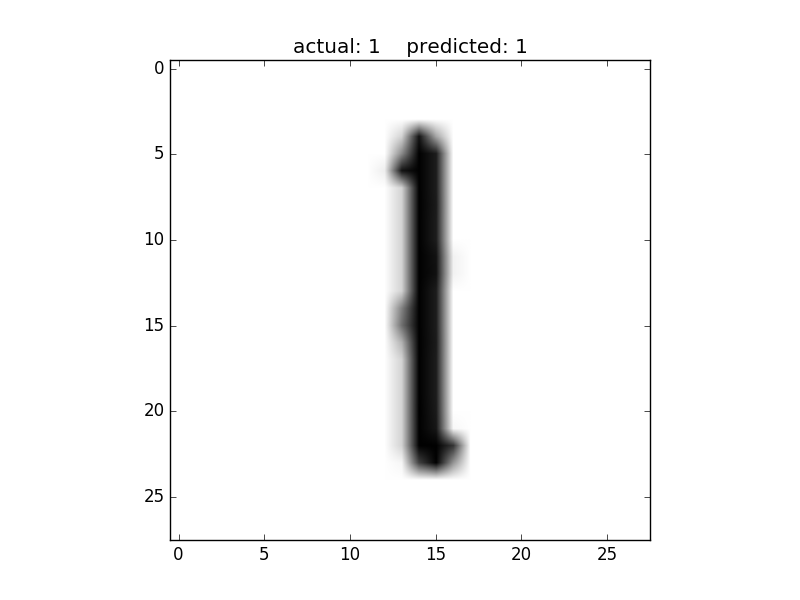
\includegraphics[width=\textwidth]{sample_original1.png}
	\end{minipage} \hfill
	\begin{minipage}{0.5\textwidth}
		\centering
		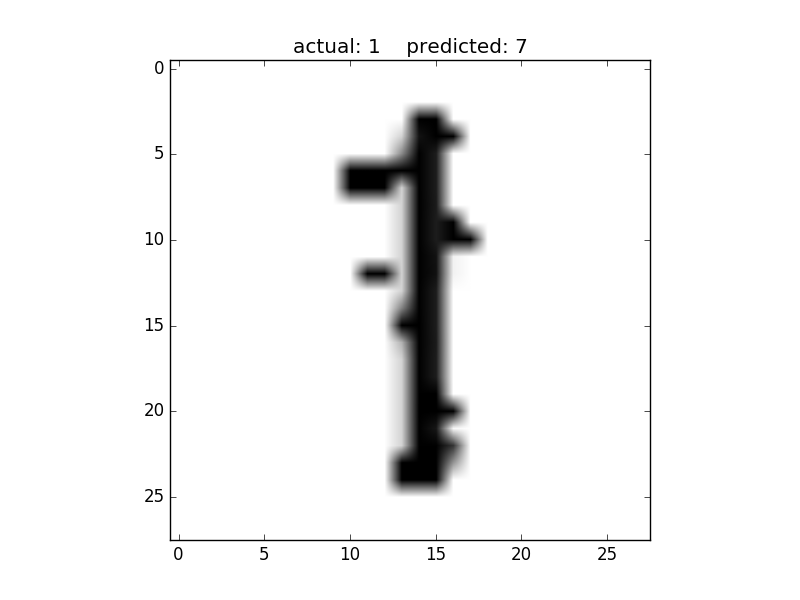
\includegraphics[width=\textwidth]{sample_perturbed1.png}
	\end{minipage} 
\end{figure}
\begin{figure}[h!]
	\begin{minipage}{0.5\textwidth}
		\centering
		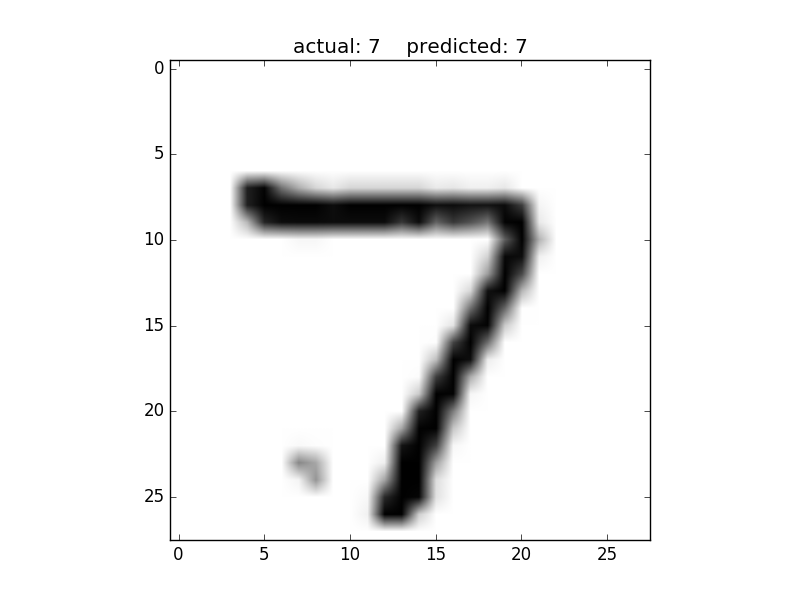
\includegraphics[width=\textwidth]{sample_original2.png}
		\caption{Original examples from MNIST}
	\end{minipage} \hfill
	\begin{minipage}{0.5\textwidth}
		\centering
		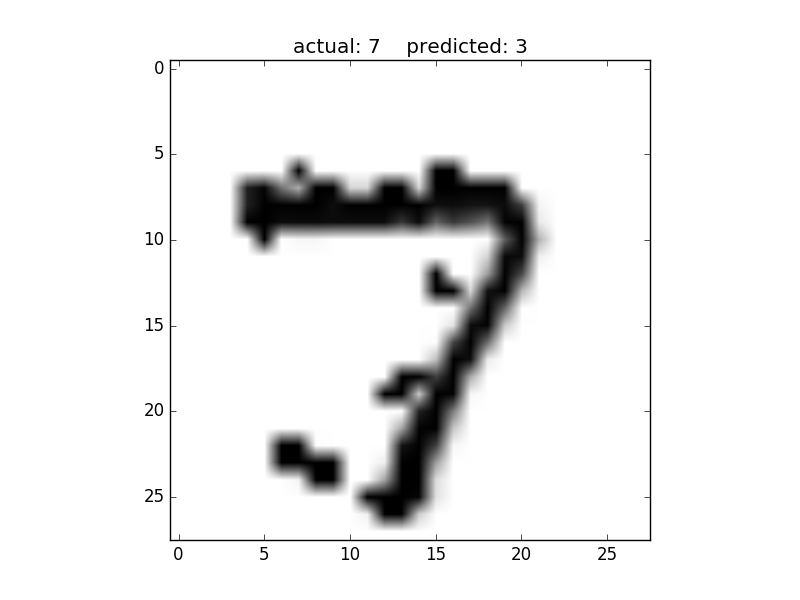
\includegraphics[width=\textwidth]{sample_perturbed2.png}
		\caption{Adversarial samples}
	\end{minipage}
\end{figure}

For traditional CNN, the success rate is $72\%$ with maximum 100 pixels perturbed using adversarial sample crafting \textbf{algorithm 1.}, more than $95\%$ by \textbf{algorithm 2.} and \textbf{algorithm 3.}.

\subsection{Adversarial Sample Crafting Algorithms}
\paragraph{Algorithm 1.}
\begin{enumerate}

\item Randomly select a sample input ( with its target output and make a copy of that input array denoted as $c$

\item Build a saliency map $S$ mapping each index $S[m][n]$ to the gradient of the cross-entropy (loss function) with respect to the corresponding input$c[m][n]$, which as a whole forms a 2D array. (see an example in \textbf{Appendix A}

\item Iterate for trial from $i=1$:

\begin{enumerate}
	\item Find the maximum number $k_i[m][n]$ in the saliency map.

	\item Set $k_i[m][n]$ to minus infinity  and $c[m][n]$ to the maximum.

	\item Feed $c$ to the trained CNN and check if the output differs from the target output:
		\begin{enumerate}
			\item Yes. terminate the loop and output i
			\item No. set $i=i+1$. If $i > 100$, terminate and output "Failed". Otherwise, go back to step \textbf{(a).}
		\end{enumerate}
\end{enumerate}
\end{enumerate}
This algorithm was proposed by Papernot\cite{Papernot} in 2016 to simplify the process of crafting adversarial samples. It focuses solely on the pixels of positive large gradient with respect to the cross-entropy, but the information contained in the pixels with negative as large gradient is left out.
In addition, this algorithm would fail when the gradient of original pixels picked by saliency map is close to the maximum.\cite{Papernot2}
Let $Grad(x_[m][n])$ be the gradient of loss function on $[m][n]$ of the input array, we have 
\begin{equation}
	\Delta loss = Grad(x[m][n])\Delta x[m][n]
\end{equation}
$\Delta loss$ would not change too much with small $\Delta x[m][n]$ even when $Grad(x[m][n])$ is large.

Therefore, we implement the following algorithm to make use of most of the information from the input array.

\paragraph{Algorithm 2.}
\begin{enumerate}
	\item Randomly select a sample input and make a copy of it as $c$, plug $c$ into the loss function $L$ and calculate the loss of the example. Denote it as $loss_0=L(c)$ and let $S_1,S_2$ represent two saliency maps.
	\item Iterate through the input array and for any $m,n$
		\begin{enumerate}
			\item $c[m][n]=temp$
			\item $c[m][n]=1(maximum)$
			\item $S_1[m][n]= \mid L(c) - loss_0 \mid$
			\item $c[m][n]=0(minimum)$
			\item $S_2[m][n]=\mid L(c) - loss_0 \mid$
			\item $c[m][n]=temp$
		\end{enumerate}

	\item Iterate for trial from $i=1$:
		\begin{enumerate}
			\item Find $M_i=max\{S_1[m][n],S_2[m][n]\}$ in the saliency map.
				\begin{enumerate}
					\item if $M_i==S_1[m][n]$, $c[m][n]=1(maximum)$
					\item if $M_i==S_2[m][n]$, $c[m][n]=0(minimum)$
				\end{enumerate}
			\item Feed $c$ to the trained CNN and check if the output differs from the target output:
				\begin{enumerate}
					\item Yes. terminate the loop and output i
					\item No. set $i=i+1$. If $i > 100$, terminate and output "Failed". Otherwise, go back to step \textbf{(a).}
				\end{enumerate}
		\end{enumerate}
\end{enumerate}

This algorithm captures most of the information in the input array as it makes use both positive and negative large gradients. It also takes into account the amplitude of the changing step for each input pixel to maximize the equation (1).

However, the computational cost or time efficiency cost is $\mathcal{O}(N+M)$ where $N$ is the length of the input array and $M$ is the limit of the number of pixels to be modified. 
But the \textbf{algorithm 1} is of $Omicron(N)$ if we assume the cost for computing gradient on a piexel the same as the cost for evaluating the loss function once.

We can actually sacrifice a little accuracy to obtain a $\mathcal{O}(N)$ efficiency.

\paragraph{Algorithm 3.}
\begin{enumerate}
\item Randomly select a sample input ( with its target output and make a copy of that input array denoted as $c$

\item Build a saliency map $S$ mapping each index $S[m][n]$ to the gradient of the cross-entropy (loss function) with respect to the corresponding input$c[m][n]$, which as a whole forms a 2D array. (see an example in \textbf{Appendix A}

\item Iterate for trial from $i=1$:

\begin{enumerate}
	\item Find the number $k_i[m][n]$ with maximum absolute value in the saliency map.

	\item Set $k_i[m][n]$ to 0 and $c[m][n]$ to the 1(maximum) if $k_i[m][n] > 0$ and 0(minimum) otherwise ($k_i[m][n] < 0$).

	\item Feed $c$ to the trained CNN and check if the output differs from the target output:
		\begin{enumerate}
			\item Yes. terminate the loop and output i
			\item No. set $i=i+1$. If $i > 100$, terminate and output "Failed". Otherwise, go back to step \textbf{(a).}
		\end{enumerate}
\end{enumerate}
\end{enumerate}

These three algorithms are implemented in our work and the code is availabale at \url{https://github.com/songhobby/CNN.git} named as test1,py, test3,py and test2.py.

Though, this is not the end of story. A more effective algorithm is to calculate the saliency map every time an index of input array is modified. But the computational cost is of $\mathcal{O}(N^2)$.
\paragraph{Algorithm 4.}
Based on \textbf{Algorithm 2.}, update the saliency maps each time an input array index is modified.
\section{Temperature vs. Distillation against Adversarial Perturbations}

\paragraph{Definition 2.}
The \textbf{temperature} of a softmax layer (usually used as an output layerin DNN) is defined as the parameter $T$ such that the softmax function with temperature becomes 
\begin{equation}
	f(\mathbf{x_i};T)=\frac{\exp{\frac{\mathbf{x_i}}{T}}}{\sum_{j=1}^n 
	\exp{\frac{\mathbf{x_j}}{T}}}
\end{equation}
We can show that as temperature increases, the robustness or sensitivity to perturbations of pixels decreases tremendously.
\paragraph{Proof 1.}
Let $\mathbf{x}$ be the input vector to the softmax output layer and the target vector $\mathbf{y}$ is a one-hot vector with $1$ at $j$, $j\in{0,1,\dots 9}$ and $0$ for the rest indices.

The loss function $L$ is, for $\mathbf{y}_k=1$:
\begin{equation}
	L(\mathbf{x}) = \frac{\exp{\frac{\mathbf{x}_k}{T}}}{\sum_{j=0}^9 \exp{\frac{\mathbf{x}_j}{T}}}
\end{equation}
\begin{align}
	\frac{\partial L(\mathbf{x})}{\partial \mathbf{x}_i} &= 
	\frac{1}{(\sum_{j=0}^9 \exp{\frac{\mathbf{x}_j}{T}})^2}
	(
	\frac{\partial \exp{\frac{\mathbf{x}_k}{T}}}{\partial \mathbf{x}_i}
	\sum_{j=0}^9 \exp{\frac{\mathbf{x}_j}{T}} 
	+ \exp{\frac{\mathbf{x}_k}{T}}
	\frac{\partial \sum_{j=0}^9 \exp{\frac{\mathbf{x}_j}{T}}}{\partial \mathbf{x}_i}
	)\\
	&=
	\frac{1}{T(\sum_{j=0}^9 \exp{\frac{\mathbf{x}_j}{T}})^2} (
	\delta (i-k) \exp{\frac{\mathbf{x}_k}{T}}
	\sum_{j=0}^9 \exp{\frac{\mathbf{x}_j}{T}}+
	\exp{\frac{2\mathbf{x}_k}{T}} )
\end{align}

The temperature as a term in denominator 


we chose the temperature at $t=20$ as it is an appropriate setting at which both relatively high prediction accuracy and robustness are achieved by papernot's empirical study\cite{Papernot}.

\newpage
\appendix
\section{Sample Saliency map for tradional CNN}
mean gradient: -2.2915e-08\\
max gradient: 9.78318e-05\\
Perturbed: 12\\
Saliency map:\\
$[[$  1.96173855e-09   1.35970735e-09  -8.05801559e-09   3.28918093e-09 \\
   -5.48783348e-08  -7.17473085e-08  -4.38453718e-08  -5.30832978e-08 \\
   -2.52357182e-07  -1.88820479e-07  -1.97611584e-07  -1.68086672e-07 \\
   -7.32964693e-08  -1.42316367e-07  -1.02478126e-07  -1.31316881e-07 \\
   -1.58633611e-07  -1.31892534e-07  -1.97597899e-07  -2.12147782e-07 \\
   -1.20857607e-07  -1.28928747e-07  -4.98595369e-08  -4.03208240e-08 \\
   -7.82443266e-09  -1.32436873e-09   0.00000000e+00   0.00000000e+00 $]$ \\
    1.95072070e-09  -7.56662510e-10  -1.79181256e-08  -3.19850635e-09 \\
   -8.84076456e-08  -7.99879629e-08  -9.83269643e-08  -2.67942539e-07 \\
   -7.58413535e-07  -6.11258770e-07  -4.33601514e-07  -2.66673595e-07 \\
    7.28429370e-08   1.23588109e-08   7.01912199e-08  -3.30841772e-08 \\
   -1.88335321e-07  -1.84600680e-07  -2.85333499e-07  -2.19011724e-07 \\
    4.65144439e-08   1.59647158e-08   9.08492268e-08   6.10932176e-08 \\
	3.85807297e-08   2.76906196e-08   0.00000000e+00   0.00000000e+00 $]$ \\
   -4.20748947e-09  -2.18477370e-09  -3.84939938e-08  -4.47094806e-08 \\
   -5.14061682e-08   1.53504047e-07   9.17623311e-08   1.04581090e-08 \\
    8.77676030e-08   4.88882733e-07   5.50281470e-07   7.53525512e-07 \\
    9.84536655e-07   4.51604876e-07   2.71482520e-07  -1.81879841e-07 \\
    5.97312351e-08   3.29956265e-07   1.50822700e-07   3.56565351e-07 \\
    8.15367969e-07   5.19170669e-07   3.63578181e-07   1.58566408e-07 \\
    1.45516594e-07   7.73982194e-08  -1.83289606e-09  -7.77444054e-10$]$ \\
 $[$ -1.02055981e-08  -1.19342607e-08  -3.08573220e-08   3.72754307e-08 \\
    2.20618276e-07   6.08017331e-07   8.38857488e-07   6.92404910e-07 \\
    1.32143373e-06   1.64081018e-06   1.69421537e-06   2.58918908e-06 \\
    4.61905483e-06   3.51893982e-06   2.39151245e-06   5.98073598e-07 \\
    1.13812894e-06   1.60477293e-06   2.00945988e-06   2.09306722e-06 \\
    2.74859985e-06   2.79267442e-06   1.30998785e-06   5.38874133e-07 \\
    1.48021627e-07   6.51662404e-08  -4.27208824e-11  -3.48784424e-09$]$ \\
 $[$ -1.44070569e-08  -1.32951321e-08   9.07851643e-08   2.17700261e-07 \\
    2.62837204e-07   4.18497734e-07   6.46274998e-07   8.14089731e-07 \\
    3.08582366e-06   8.33536069e-06   1.30672488e-05   7.04140575e-06 \\
   -2.41726229e-06  -1.07430587e-05  -1.45426056e-05  -5.74765818e-06 \\
    1.78234131e-07   1.19687093e-06   1.99419901e-06   3.59732940e-06 \\
    6.97585074e-06   5.88091916e-06   2.81491452e-06  -7.44247046e-08 \\
    4.02008197e-07   1.79280406e-07   5.18654453e-10  -2.27380781e-10$]$ \\
 $[$  1.39619694e-08   7.94599799e-08   2.30915077e-07   1.45152370e-07 \\
   -1.62453290e-07   4.98938050e-07   1.09356279e-06   3.30207649e-06 \\
    5.32647027e-06   1.17240131e-06  -2.52363971e-05  -3.77056786e-05 \\
   -2.10110920e-05   2.28969529e-05   5.51288531e-06  -7.51445987e-06 \\
   $\dots \dots \dots ]]$

\newpage
\bibliography{Papernot,Papernot2,MNIST,Lasagne,Theano} 
\bibliographystyle{IEEEtran}
\end{document}
